% Chapter 2

\chapter{Literature Review} % Main chapter title

\label{Chapter2} % For referencing the chapter elsewhere, use \ref{Chapter1}

%----------------------------------------------------------------------------------------

% Define some commands to keep the formatting separated from the content

%----------------------------------------------------------------------------------------

\section{Cellular Automata and Game of Life}
Cellular Automata can be modelled in a number of dimensions including anything from one, two, three, four, or more dimensions.\citep{adamatzky2010game} In this project the focus will be on the two dimensional approach using a \textsl{n}-dimensional lattice (will be referred to as a grid). The grid can be of infinite size, however will be limited to a finite space i.e. a predetermined set of cells superimposed over a map of an informal settlement.\\\\
An individual square in the grid (which will be referred to as a cell) can have upto eight neighbours. This is shown in the diagram below.
\begin{figure}[H]
\centering
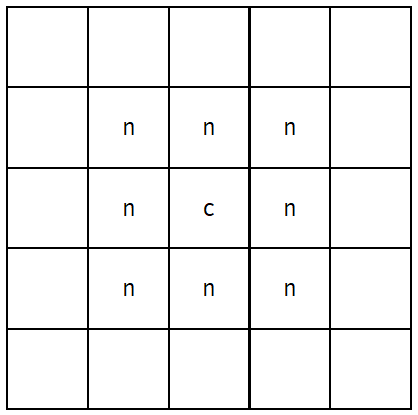
\includegraphics[scale=0.5]{Figures/cell.png}
\caption{A cell 'c' and its neighbours 'n'}
\label{fig:cell}
\begin{center}
Source: Own Creation (2021)
\end{center}
\end{figure}
A cell can have two discrete states for any given discrete time unit (referred to as generation). These states can be 'alive' or 'dead'. A cell is shown to be alive by having it \textsl{shaded} and if it is dead it is left blank.\citep{adamatzky2010game} This is shown in the figure below.
\begin{figure}[H]
\centering
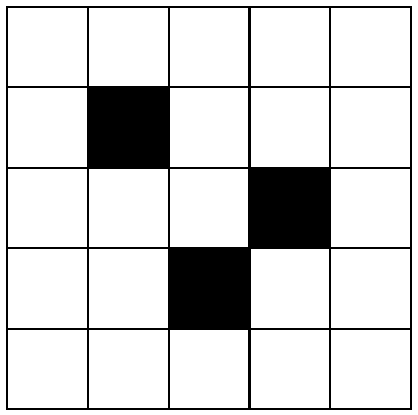
\includegraphics[scale=0.5]{Figures/shaded.png}
\caption{A grid showing alive and dead cells}
\begin{center}
Source: Own Creation (2021)
\end{center}
\end{figure}
As shown in Figure \ref{fig:cell} a cell can have either lateral or diagonal neighbours. The rules of \textsl{Life} were discussed briefly above in Section \ref{sec:prob}. A graphical representation of these is shown below.
\begin{figure}[H]
\centering
\begin{subfigure}{.5\textwidth}
  \centering
  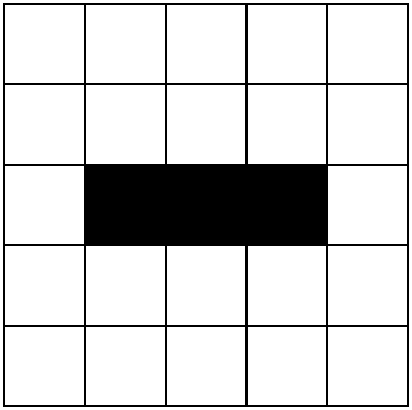
\includegraphics[width=.4\linewidth]{Figures/blink1.png}
  \caption{Generation $t = 0$}
\end{subfigure}%
\begin{subfigure}{.5\textwidth}
  \centering
  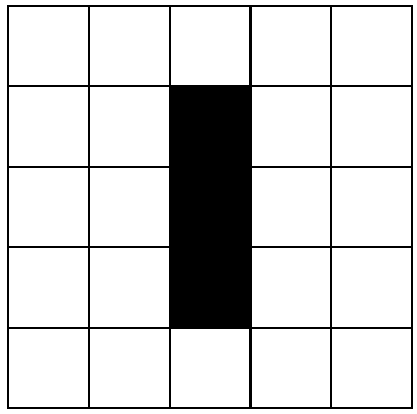
\includegraphics[width=.4\linewidth]{Figures/blink2.png}
  \caption{Generation $t = 1$}
\end{subfigure}
\caption{A simple 2 generation iteration of \textsl{Life}}
\begin{center}
Source: Own Creation (2021)
\end{center}
\end{figure}
Another slightly more advanced setup of \textsl{Life} is shown below.
\begin{figure}[H]
\centering
\begin{subfigure}{.5\textwidth}
  \centering
  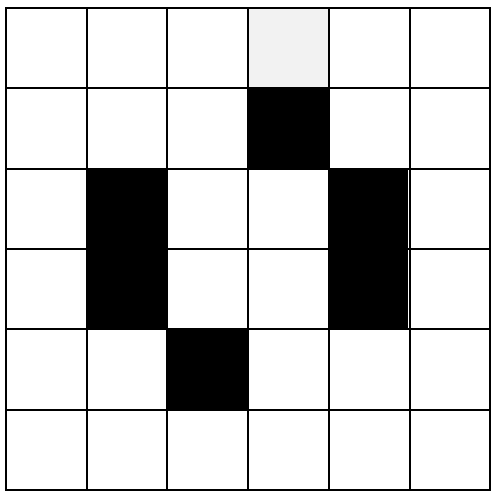
\includegraphics[width=.4\linewidth]{Figures/toad1.png}
  \caption{Generation $t = 0$}
\end{subfigure}%
\begin{subfigure}{.5\textwidth}
  \centering
  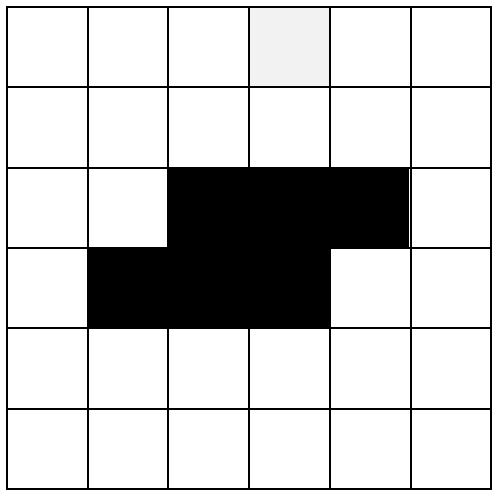
\includegraphics[width=.4\linewidth]{Figures/toad2.png}
  \caption{Generation $t = 1$}
\end{subfigure}
\caption{An advanced 2 generation iteration of \textsl{Life}}
\begin{center}
Source: Own Creation (2021)
\end{center}
\end{figure}
In a seminal paper by Stephen Wolfram, four classes of CA were proposed according to their behaviour given an initial random condition .\citep{Wolfram1984} These four classes are as follows:
\begin{itemize}
\item Class 1 - After a finite number of generations a unique homogeneous state is reached i.e. all cells become the same eventually.
\item Class 2 - Simple structures are generated which are either periodic, or stable (also called persistent).
\item Class 3 - An aperiodic (or chaotic) patterns emerge which carry on indefinitely.
\item Class 4 - Capable of universal computations i.e. can exhibit complex behaviour. 
\end{itemize}
Due to the nature of the rules of \textsl{Life} certain patterns emerge. This is thanks to the cycles of repeated stated which evolve over certain number of generations. These patterns include still-lifes, period two (or \textsl{blinkers}), gliders, oscillators, glider guns, and puffer trains.\citep{adamatzky2010game}
\\\\
The applications of CA and, or \textsl{Life} have sparked a number of research papers in fields such as physics, music, complexity, and computation. \\
Examples in physics include, interaction between a complex system and electromagnetic radiation \citep{conti}, an implementation of \textsl{Life} with quantum features.\citep{quantum}\\
Implementations in music include the development of CAMUS (\textbf{C}ellular \textbf{A}utomata \textbf{Mus}ic).\citep{music}\\
In the fields of complexity, and computation a vast array of work has been done therefore a few examples include; Universal Computer-Constructor in CA \citep{gou}, and creation of a Turing Machine in \textsl{Life}.\citep{ren}
\section{Informal settlements}
Informal settlements are housing dwellings that are part of urban districts or neighbourhoods that arise and develop without oversight or control from the state. They are synonymous with 'slums' or 'squatters', though are not the same. They form an integral element of urban sustainability whereby developing cities can not develop without them. The connotations with 'informal', 'slums', and 'squatter' have always been seen in a negative light. This is not seen as beneficial as the growth of urbanisation is highly intertwined with informal settlements.\citep{dovey2011forms}\\
Across the globe informal settlements are known colloquially by their own variety of terms. \citep{un} In this project the umbrella term informal settlement will be utilised.\\
The process or principles of informal settlements growth can be grouped into three categories namely;\citep{dovey2011forms}
\begin{itemize}
\item \textsl{settling} - simply settling down on what is usually unclaimed land
\item \textsl{inserting} - usually into urban areas that are abandoned, or uninhabited
\item \textsl{attaching} - informal settlements that grow out of existing urban settlements
\end{itemize}
In morphological terms, informal settlements can be classified into eight different types. This refers to the urban conditions rather that the process mentioned above, however it is not to say that the two are mutually exclusive. The types are not mutually exclusive from each other either. The types are as follows:\citep{dovey2011forms}
\begin{itemize}
\item Districts - most popular where over long periods of time the settlement grows to encompass mixed-use districts with both retail, and industrial functionality.
\item Waterfronts - settlements between land and water, whether it is a lake, harbour, river, canal to name a few. Prone to water issues such as flooding if the climate is such.
\item Escarpments - settlements on urban topography that is usually too steep to build formal structures. an example location would be an area between a mountain and a city. Can be prone to earthquakes, landslides, and mudslides if the climate is such. Transportation is another key concern.
\item Easements - Major infrastructure in urban cities such as roads, railways, pipelines to name a few offer \textsl{'buffer'} zones which can become informal settlements.
\item Sidewalks - These settlements emerge when public area such as sidewalks have an area where people can set up dwellings, even if for temporary usage.
\item Adherences - Related to the principle mentioned above.
\item Backstages - Settlements hidden from the public's gaze. Becomes more informal the \textsl{'deeper'} one goes from a formal street frontage.
\item Enclosures - Settlements where the \textsl{'shell'} is contained with in another urban building.
\end{itemize}
Informal settlement residents just like the residents of formal settlements have a desire for a good quality of life. Factors that influence this quality of life include food storage and preparation, water, sanitation, air quality and pollution, electricity, health risks, access to public facilities and amenities, among other things.\citep{richards2007measuring}\\
Richards et al. (2007), further sates that everyday problems such as unemployment, and crime also influence the quality of life. The paper further stipulates that the research can be expanded further to look into spatial and temporal factors that influence informal settlements.\\\\
The characteristics of informal settlements transcend the physical and are closely knitted with socio-economic as well as political conditions.\citep{wekesa}
\section{Modelling Urban Development}
The phenomenon of urbanisation in the last century has drastically increased from a mere 13\% in 1900 to a 49\% in 2005. The current projected estimates for the year 2030 in 60\%. The majority of this urbanisation is still going to occur in the developing nations.\citep{un2005}\\\\
One of the three factors that is going to influence humans directly in the near future is the land-use/land cover change. This will affect policy makers, geographers, and planners all alike. This is thanks to the socio–environmental consequences of the spatio-temporal process of urban development.\citep{vitousek1994beyond,liu2008modelling}\\\\
When it comes to geographic models they can be categorised into three categories of increasing abstraction.\citep{thomas1980modelling} The models are as follows:
\begin{itemize}
\item Scale
\begin{itemize}
\item Iconic
\item Analogue
\end{itemize}
\item Conceptual or Diagrammatical
\item Mathematical
\begin{itemize}
\item Probability
\item Deterministic 
\end{itemize}
\end{itemize}
The mathematical models are therefore the highest level of abstraction. Scale models mimic reality but are miniaturised copies of the real world. The main difference between Iconic and Analogue is the later besides being replicas they tend to transform certain properties of the real world system, e.g. using wool for clouds. Conceptual models are concerned with the relationships that exist between components in the system e.g. a sewage system can be denoted with arrows and boxes on a diagram. Mathematical models if in their purest form translate a conceptual model in to pure, formal, and symbolic logic of mathematics.\citep{thomas1980modelling}\\\\
The flow chart of the modelling process is shown below.
\begin{center}
\begin{tikzpicture}[node distance=2cm]
\node (start) [startstop] {Beginning};
\node (pro1) [process, below of=start] {Identify problem in the real-world};
\node (pro2) [process, below of=pro1] {Set-up and formulate model};
\node (pro3) [process, below of=pro2] {Implement model in a program};
\node (pro4) [process, below of=pro3] {Calibrate and refine outcome};
\node (pro5) [process, below of=pro4] {Satisfactory outcome?};
\node (stop) [startstop, below of=pro5] {Modelling process complete};
\node (no) [startstop, right of=pro5, xshift=3cm] {No};
\draw [arrow] (start) -- (pro1);
\draw [arrow] (pro1) -- (pro2);
\draw [arrow] (pro2) -- (pro3);
\draw [arrow] (pro3) -- (pro4);
\draw [arrow] (pro4) -- (pro5);
\draw [arrow] (pro5) -- (stop);
\draw [arrow] (pro5) -- node[anchor=east] {yes} (stop);
\draw [arrow] (pro5) -- (no);
\draw [arrow] (no) |- (pro1);
\end{tikzpicture}
\\Source: Own Creation (2021) adapted from \citep{liu2008modelling}
\end{center}
Before continuing it should be noted that one of the major pitfalls of models are they are a simplified view of reality, hence they can tend to leave certain facts behind of reality.\citep{liu2008modelling}\\\\
One of the earliest models created in geography and urban modelling dates back to the 1800s where Johann Heinrich von Th{\"u}nen in his book titled \textsl{Der isolierte Staat} translated to mean \textsl{The Isolated State} discussed maximising agricultural production.\citep{clark1967thunen}\\
Other seminal research included the like of Alfred Weber in the early 1900s published the title \textsl{{\"U}ber den Standort der Industrien} which translates to \textsl{Theory of the Location of Industries} This work created models based on real-world conditions.\citep{fearon2006alfred}